\documentclass[a4paper,oneside]{Tptesi2}

\usepackage[italian]{babel}
\usepackage{listings}
\usepackage{amsmath,amssymb}
\usepackage{verbatim}
\usepackage{indentfirst}
\usepackage[utf8]{inputenc}
\usepackage{subfigure}
\usepackage{algorithmic}
\usepackage{framed}
\usepackage{rotating}
\usepackage{cite}
\usepackage{url}
\usepackage{hyperref}

% Packages -----------------------------------------------------------------------
%\usepackage{amsthm}
%\usepackage{amsmath}          % Non necessario se usi TPTESI2 perche' gia` incluso
%\usepackage[dvips]{graphicx}  % Non necessario se usi TPTESI2 perche' gia` incluso
%\usepackage{url} %non usare se si usa hyperref


\newcommand{\mr}{\emph{motore di ricerca}}
\newcommand{\Mr}{\emph{Motore di ricerca}}
\newcommand{\ws}{Web~service }


% Use a small font for the verbatim environment
\makeatletter  % makes '@' an ordinary character
\renewcommand{\verbatim@font}{%
  \ttfamily\footnotesize\catcode`\<=\active\catcode`\>=\active%
}
\makeatother   % makes '@' a special symbol again
%
% Simboli Matematici -------------------------------------------------------------
%\newcommand{\h}{\mathcal{H}_\infty} % scorciatoia per sequenza usata spesso
% Definizioni & Teoremi ----------------------------------------------------------
\newtheorem{teorema}{Teorema}[chapter]
\newtheorem{corollario}[teorema]{Corollario}
\newtheorem{lemma}[teorema]{Lemma}
%\theoremstyle{definition}
\newtheorem{definizione}{Definizione}[chapter]
\newtheorem{proposizione}[definizione]{Proposizione}
% Formattazione Figure -----------------------------------------------------------
\setcounter{topnumber}{3}
\setcounter{totalnumber}{3}
\def\topfraction{1}
\def\textfraction{0}
% Fuzz ---------------------------------------------------------------------------
%\hfuzz10cm %Non scassare linee che escono dal bordo
% Frontespizio -------------------------------------------------------------------
       \title{Continual Learning : Visual Recognition per Problemi con Task Incrementali}
       \author{Lorenzo Gianassi}
       \titolocorso{Ingegneria Informatica}
       \chair{Andrew D. Bagdanov}
       \numberofmembers{1} %numero dei relatori
       \degreeyear{2019/2020}
       \numerocorrelatori{2} %numero dei correlatori
       \correlatori{insert correlators\ldots} % i correlatori separati da \\

%
% ---- Inclusioni (vedi piu` sotto per il comando "include" --------------
%\includeonly {introduzione,chapter1, chapter2}
%\includeonly {chapter1, chapter2, chapter3, chapter4, chapter5, chapter6}
%\includeonly{chapter6}
%
\hypersetup{%
%  pdfpagemode=FullScreen,%
  plainpages=false,%
  breaklinks,%
  pdftitle={},%
  pdfauthor={},%
  pdfsubject={},%
  pdfkeywords={},%
  colorlinks=false}

\begin{document}

\frontmatter

%\hyphenation{}
%
\pagestyle{headings} % rende attive le impostazioni sulla testata!
%
\maketitle % crea il frontespizio (ricordati di copiare "stemma.eps" nella tua directory)
%
%
%\pagenumbering{roman}
\tableofcontents % inserisce indice generale
\cleardoublepage
%\addcontentsline{toc}{chapter}{Elenco delle figure}
%\listoffigures   % inserisce indice figure
%\addcontentsline{toc}{chapter}{Elenco delle tabelle}
%\listoftables    % inserisce indice tabelle
%\addcontentsline{toc}{chapter}{Elenco degli algoritmi}
%\listofalgorithms
%
%--------------- Inizio del testo vero e proprio
%

%\cleardoublepage
%\pagenumbering{arabic}
%\input{files/ringraziamenti}
\frontmatter
\chapter{Introduzione}\label{ch:introduzione}
\section*{Motivazioni}
Gli esseri umani e gli animali hanno la capacità di acquisire, perfezionare e modificare continuamente le proprie conoscenze e abilità per tutta la durata della loro vita. Questa capacità, chiamata \textit{Continual Learning}, è composta da una ricca serie di meccanismi \textit{neurocognitivi} che insieme contribuiscono allo sviluppo e alla specializzazione delle nostre abilità sensomotorie, nonché al rafforzamento e al recupero della memoria a lungo termine. Di conseguenza, l'applicazione del \textit{Continual Learning} a  \textit{sistemi computazionali} e \textit{agenti autonomi} che interagiscono nel mondo reale ed elaborano flussi continui di informazioni può essere di  fondamentale importanza. Tuttavia, il \textit{Continual Learning} rimane una sfida di lunga data per il \textit{Machine Learning} e i modelli di \textit{Rete Neurale} poiché l'acquisizione continua di informazioni disponibili in modo incrementale da distribuzioni di dati non stabili generalmente porta ad ottenere il \textit{Catastrophic Forgetting}, concetto che andremo a definire successivamente.\newline
Questo rappresenta un grave problema per i modelli di \textit{Rete Neurale} moderni che in genere apprendono rappresentazioni da \textit{batch} stazionari di dati di \textit{Training}, quindi senza tenere conto delle situazioni in cui le informazioni diventano disponibili. Di conseguenza, la capacità  di apprendere da un flusso continuo  senza avere una perdita di memoria sui dati precedenti potrebbe avvicinare l'apprendimento delle \textit{reti neurali} a quello dell'essere umano con sviluppi interessanti per la scienza.
\section*{Presentazione del Lavoro}
In questo elaborato di tesi, partendo dal lavoro di \cite{Continual_Learning}, verrà descritto il concetto \textit{Continual Learning} mostrandone i pregi e le difficoltà(\textit{Catastrophic Forgetting}) tramite un problema di \textit{Visual Recognition}. Per fare ciò è stato implementato un \textit{framework} che fosse in grado di eseguire una \textit{Pipeline}, che avrà il compito di eseguire l'apprendimento svolto da un modello per il \textit{Continual Learning} mostrando l'occorrere del \textit{forgetting}. Prima di mostrare i risultati ottenuti verranno descritti i concetti a livello teorico e presentati gli strumenti utilizzati durante la \textit{Pipeline}.\newline
Il lavoro descritto è diviso in tre parti: la prima relativa al \textit{Joint-Train} e le ultime due alle configurazioni \textit{Task Agnostic/Task Aware}. Successivamente, sarà presentata una soluzione molto \textit{naïve} ispirata dal \textit{paper} \cite{Continual_Learning}.


\mainmatter
\chapter{Definizioni}\label{ch:chapter1}
In questo capitolo andiamo a introdurre i concetti principali su cui si basa l'elaborato, che ci serviranno successivamente per apprezzarne l'utilità. 
\section{Continual Learning}
Negli ultimi anni i modelli del \textbf{Machine Learning} sono stati addirittura in grado di sorpassare l'intelletto umano per svariati problemi, come ad esempio il \textbf{Visual Recognition}.
Sebbene questi risultati siano sorprendenti, sono stati ottenuti con modelli statici non in grado di espandere il loro comportamento o adattarlo nel tempo. Si introduce quindi il concetto del \textbf{Continual Learning} su cui si basa questo elaborato.\newline
\textit{Continual Learning} mira a creare algoritmi di\textit{Machine Learning} in grado di accumulare un insieme di conoscenze apprese sequenzialmente. L'idea generale alla base di quest'ultimo è rendere gli algoritmi in grado di apprendere da una fonte di dati reale. In un ambiente naturale le opportunità di apprendimento non sono disponibili contemporaneamente e devono essere elaborate in sequenza.\newline
Il \textbf{Continual Learning} studia il problema dell'apprendimento da uno \textit{stream} infinito di dati, con l'obbiettivo di estendere gradualmente la conoscenza e di usarla per allenamenti successivi. La dimensione dello \textit{stream} di dati ed il numero di \textit{tasks} su cui si lavora non è necessariamente noto a priori.  Il \textit{Continual Learning} può essere anche definito come \textbf{Lifelong Learning}, \textbf{Sequential Learning} o \textbf{Incremental Learning}.
Il concetto fondamentale su cui si basa  è la natura sequenziale del processo di apprendimento, in cui solo una porzione dei dati di input di uno o più \textit{tasks} è disponibile in quell'istante di tempo.
\section{Catastrophic Forgetting}
Come viene introdotto in \cite{Continual_Learning}, una rete neurale \textit{dimentica} quando le sue prestazioni su una distribuzione dati vengono ridotte dall'apprendimento su una successiva.
La sfida maggiore del \textit{Continual Learning} consiste nell'apprendere evitando il  \textbf{Catastrophic Forgetting}, cioè la performance di previsione su dati appartenenti a \textit{tasks} precedentemente visionati nel training non dovrebbe calare nel tempo in seguito all'aggiunta di nuovi \textit{tasks}.
Definiamo adesso il \textbf{Catastriphic Forgetting}, noto anche come \textbf{Catastrophic Interference}, come la tendenza di una rete neurale artificiale a dimenticare completamente e in modo improvviso le informazioni apprese in precedenza dopo aver appreso nuove informazioni (come viene definito in \cite{Continual_Learning}).
\section{Stability-Plasticity Dilemma}
Per sopperire al \textbf{Catastrophic Forgetting} i sistemi di apprendimento devono, da una parte , mostrare la capacità di acquisire nuova conoscenza e affinare quella già esistente sulla base di un input continuativo, dall'altra, impedire alla nuova informazione di interferire con la conoscenza pregressa.
Il concetto  per il quale un sistema sia in grado di essere "\textit{plastico}" per l'integrazione di nuove informazioni e "\textit{stabile}"
in modo da non interferire \textit{catastroficamente} con la conoscenza precedentemente consolidata è definito con il nome \textbf{Stability-Plasticity Dilemma}.\newline
Come viene descritto in \cite{stability/plasticity} , troppa "plasticità" farà sì che i dati precedentemente codificati siano costantemente dimenticati, mentre troppa "stabilità" impedirà la codifica efficiente di questi dati a livello delle sinapsi.
\section{Task Agnostic-Task Aware}
Un concetto importante su cui si basa l'esecuzione del mio programma che simula il \textbf{Continual Learning} è la dualità di approccio \textbf{Task-Agnostic/Task-Aware}.
Definiamo un approccio \textbf{Task-Agnostic} quando la rete non conosce bene i limiti dei \textit{tasks}, cioè non conosciamo a quale \textit{task} appartenga la \textit{label} del dato in input alla \textbf{Rete Neurale Convoluzionale}. Mentre, nell'altro caso, l'approccio  \textbf{Task-Agnostic} è contraddistinto dalla nozione del \textit{task} corrente a cui appartiene il dato in input.\newline
Questi due approcci ci consentono di ottenere risultati diversi sotto l'aspetto dell'\textit{accuracy} della rete, sia durante che al termine del ciclo previsto per vedere tutti i \textit{tasks}. In particolar modo noi possiamo avere per entrambi sia il processo di \textbf{training} che quello di \textbf{testing}, ottenendo sostanzialmente quattro combinazioni di possibili processi.\newline
Vedremo successivamente come sarà possibile simulare queste due tipologie di \textit{training/testing} tramite il metodo \textit{set\_tasks} della classe che rappresenta la 
\textbf{rete neurale convoluzionale}.

\chapter{Componenti del Progetto}\label{ch:chapter2}
TUTTE LE INFORMAZIONI LE HO PRESE DA WIKIPEDDIA E DAI DOCS DI PYTORCH
\section{PyTorch}
\textbf{PyTorch} è una libreria di \textit{Machine Learning} open source basata sulla libreria \textbf{Torch}, utilizzata per applicazioni come la visione artificiale e l'elaborazione del linguaggio naturale, sviluppata principalmente dal laboratorio di ricerca AI di Facebook.È un software gratuito e open source nato  per essere utilizzato con il linguaggio di Programmazione Python(come avviene in Questo Elaborato), PyTorch ha anche un'interfaccia C ++.
Ho utilizzato questa librearia perchè fornisce due specifiche molto utili per lavorare con le Reti Neurali:\textit{Pytorch Tensor} e i Moduli (AutoGrad ,Optim, nn).
PyTorch definisce una classe chiamata Tensor (torch.Tensor) per memorizzare e operare su array di numeri rettangolari multidimensionali omogenei.
\newpage
\subsection{PyTorch Tensor}
I tensori PyTorch sono simili agli array NumPy, ma possono essere utilizzati anche su una GPU Nvidia compatibile con CUDA. Per Lavorare al \textbf{Visual Recognition} è molto utile lavorare su GPU: I tempi e le perfomance ne risentono in positivo.
\subsection{Moduli}
PyTorch utilizza un metodo chiamato \textit{automatic differentiation}(\textbf{AutoGrad Module}). Un \textit{Recorder} registra le operazioni eseguite, quindi le riproduce all'indietro per calcolare i gradienti. Questo metodo è particolarmente potente quando si costruiscono reti neurali per risparmiare tempo in un'epoca calcolando la differenziazione dei parametri nel passo del \textit{Forward}.
\newline
Il secondo Modulo che ci interssa è \textbf{Optim Module}(\textit{torch.optim}).
È un modulo che implementa vari algoritmi di ottimizzazione utilizzati per la creazione di reti neurali. La maggior parte dei metodi più utilizzati sono già supportati, quindi non è necessario crearli da zero. In particolare l'algortimo di Ottimizzazione che ho utilizzato in questo elaborato è \textit{optim.Adam} il quale implementa lo stochastic gradient descent.
Durante il Training si utilizzeranno i metodi della classe optim come \textit{ .zero\_grad()} e successivamente \textit{.step()} per fare l'update dei parametri della rete.
\newline
Infine Abbiamo il Modulo \textbf{\textit{torch.nn}} che ci fornisce molte più classi  per implementare e addestrare la \textit{Rete Neurale}. In particolare ci aiuta nella definizione della \textit{Rete Neurale}, e in quella dei layers che la formano.
\newpage
I Package utilizzati in questo elaborato sono:
\begin{itemize}
    \item \textit{torch.nn.Module}: È una classe base per tutti i moduli di \textit{Rete Neurale}
    \item \textit{torch.nn.Linear}: utilizzato per i layer \textit{Fully Connected}
    \item \textit{torch.nn.Conv2d}:utilizzato per i \textit{Layer Convoluzionali}
    \item \textit{torch.nn.MaxPool2d}:Viene utilizzato per applicare un max pooling 2D 
    \item \textit{torch.nn.ReLU}:Funzione di attivazione dei layer
    \item \textit{torch.nn.CrossEntropyLoss}: funzione per il calcolo della \textit{Loss} della Rete
\end{itemize}
\section{Dataset} 
\subsection{CIFAR-10}
Il Dataset utilizzato in questo elebaorato è \textbf{CIFAR-10}.
Il Dataset \textbf{CIFAR-10} è costituito da 60000 immagini a colori (avranno 3 canali per ciascuna immagine per gestire l'RGB) 32x32 divise in 10 classi, con 6000 immagini per classe. Sono disponibili 50000 immagini di allenamento e 10000 immagini di prova.\newline
Il Dataset è suddiviso in cinque batch di Training e un batch di Testing, ciascuno con 10000 immagini. Il batch di prova contiene esattamente 1000 immagini selezionate casualmente da ciascuna classe. I batch di Training contengono le immagini rimanenti in ordine casuale, ma alcuni di essi possono contenere più immagini di una classe rispetto a un'altra. In  particolare, i batch di Training contengono esattamente 5000 immagini di ciascuna classe.
\newpage
In questa immagine possiamo notare le dieci Classi di \textbf{CIFAR-10} oltre a diei esempi presi in maneira casuale da ciascuna classe.
\begin{figure}[ht]
\centering
\caption{Classi di CIFAR-10}
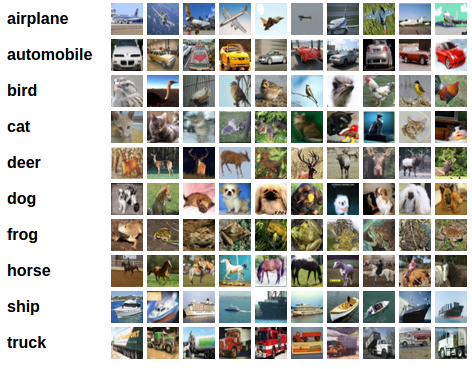
\includegraphics[width=\linewidth]{CIFAR.png}
\label{figure : CIFAR-10}
\end{figure}

\subsection{Gestione del Dataset}
Alla base della gestione dei \textit{Dataset} vi è la classe \textit{torch.utils.data.DataLoader}.
In Particolare tutti  sono sottoclassi di torch.utils.data.Dataset, ovvero hanno implementati i metodi \textit{getitem()} e \textit{len()}.
\newline
Per gestire il Dataset \textbf{CIFAR-10} ho istanziato nel mio progetto una classe \textit{Filtered\_dataset} che si occcupasse di questa mansione.
L'obbiettivo del mio elaborato era rappresentare il problema del \textbf{Continual Learning} e per fare ciò è necessario dividere il dataset utilizzato in \textit{Tasks}.
Ciò significa che a seconda del numero di \textit{Tasks} che io voglio utilizzare per simulare il \textbf{Continual Learning}
dovrò dividere il Dataset per \textit{Label}. Ad Esempio se io volessi utilizzare 5 \textit{Tasks}, per ognuno di essi avrei 2 \textit{Label}.\newline
La classe \textit{Filtered\_dataset} si occupa di creare un Subset con con il metodo della libreria di \textbf{PyTorch} \textit{torch.utils.data.Subset} che crea un subset del Dataset originario.\newline
Nel processo di suddivisione del Dataset è stato necessario \textit{mappare} le labels del dataset in modo tale da essere coerenti con l'output dell Rete. In particolare ciò è stato fatto tramite due attributi della classe \textit{Filtered\_dataset}:\textit{original2task} e \textit{task2original}. Questi due attributi consistono in due dizionari con chiave-valore le label e la rispettiva mappatura.
Ho reso inlotre possibile \textit{randomizzare} le label all'interno di ciascun task per poter fare ulteriori test con il metodo \textit{idx\_tasks}.
\newline
\section{Rete Neurale Convoluzionale}
La \textbf{Rete neurale Convoluzionale} (CNN o ConvNet) è una classe di \textit{Reti Neurali} profonde, molto spesso  applicata all'analisi ed al riconoscimento delle immagini.
La \textbf{Rete neurale Convoluzionale} che ho utilizzato in questo progetto è formata da sei \textit{Conv2D} layers separati da due \textit{MaxPool2D} ed infine da due \textit{Fully Connected Layer} sui cui ho applicato \textit{Dropout} per limitare l'\textit{Overfitting} durante il Training.
\newline
La particolarità di questa rete è che il layer dell'output è \textbf{\textit{Dinamico}}, cioè che cambia a seconda del numero di \textit{tasks} su cui si vuole lavorare e sulla tipologia di approccio scelto tra \textit{Task-Agnostic} e \textit{Task-Aware}.\newline
In Particolare è possibile aggiungere nuovi layer di output con il metodo\textit{add\_task} che richiama semplicemnte il metodo \textit{add\_module} della classe \textit{nn.Module}.
Un altro metodo importante della \textit{Rete Neurale} sarà  \textit{set\_tasks} che mi permette di settare il numero di tasks che voglio avere come output. I due attributi fondamentali della classe \textit{net} sono \textit{task\_fcs} e \textit{current\_tasks}, che sono sostanzialmente due Array contenenti gli indici dei \textit{tasks}. Il primo conterrà tutti i layer lineari per le varie  \textit{Classification Head}, mentre il secondo, seleziona quale(i) task(s) sono correntemente attivi.
Qui di seguito riporto la \textit{Rete Neurale} per un singolo task con tutte le classi corrispondente al \textit{Joint Training}:

\newline
Net(\\
  (conv1): Conv2d(3, 32, kernel_size=(3, 3), stride=(1, 1), padding=(1, 1))\\
  (conv2): Conv2d(32, 64, kernel_size=(3, 3), stride=(1, 1), padding=(1, 1))\\
  (conv3): Conv2d(64, 64, kernel_size=(3, 3), stride=(1, 1), padding=(1, 1))\\
  (pool): MaxPool2d(kernel_size=2, stride=2, padding=0, dilation=1, ceil_mode=False)\\
  (conv4): Conv2d(64, 128, kernel_size=(3, 3), stride=(1, 1), padding=(1, 1))\\
  (conv5): Conv2d(128, 128, kernel_size=(3, 3), stride=(1, 1), padding=(1, 1))\\
  (conv6): Conv2d(128, 256, kernel_size=(3, 3), stride=(1, 1), padding=(1, 1))\\
  (fc1): Linear(in_features=16384, out_features=120, bias=True)\\
  (fc2): Linear(in_features=120, out_features=84, bias=True)\\
  (dropout): Dropout(p=0.5, inplace=False)\\
  (task0\_fc): Linear(in_features=84, out_features=10, bias=True)\\
)
\newpage
Il layer \textit{Task0\_fc} è l'ultimo layer che è stato aggiunto con \textit{add\_task} e \textit{settato} con \textit{set\_task}.
Se l'esperimento fosse stato condotto su più \textit{Tasks} ci sarebbero stati altri layers oltre a \textit{Task0\_fc}. Nel caso in cui l'output voluto fosse stato su più tasks, nel metodo \textit{Forward} della rete tramite \textit{torch.cat}, sarebbero stati concatenati tra di loro i parametri corrispondenti selezionati da \textit{current\_tasks}.
\newline
La \textit{funzione di Attivazione} utilizzata nei layer \textit{Convoluzionali} è \textbf{ReLu}, come anticipato precedentemente.
La \textbf{rectified linear activation function} o \textbf{ReLU} in breve è una funzione lineare a tratti che darà  come output direttamente l'input se è positivo, altrimenti produrrà zero. L'utilizzo della \textbf{ReLu} consente di ottenere un \textit{Training} e una performance migliori.
\newline
Per quanto riguarda la funzione che si occupa del calcolo della \textit{Loss} ho optato per utilizzare la \textbf{CrossEntropyLoss}. Questa Funzione combina in una unica classe \textit{nn.LogSoftmax()} e \textit{ nn.NLLLoss()}.
Come anticipato nel paragrafo relativo a \textbf{PyTorch} ho utilizzato come \textit{optimizer} \textbf{Adam} con \textit{Learning Rate} pari a  \mathbf{0.0005}.\newline
Infine, ho reputato necessario applicare \textbf{Dropout} ai due \textit{Fully Connected Layer} che precedono il layer di output dinamico. Durante il \textit{Training}, azzera in modo casuale alcuni degli elementi del tensore di input con probabilità p utilizzando campioni da una distribuzione di Bernoulli. In questo modo ho diminuito L'\textit{Overfitting}  riscontrato sull \textit{Rete}.
\chapter{Esperimento e Risultati}\label{ch:chapter3}
\section{Introduzione al Progetto}
Prima di poter iniziare a mostare il progetto è necessario porre delle basi e limiti per quest'ultimo.
Per analizzare il problema del \textbf{Continual Learning} ci concentreremo su problemi di \textit{classificazione} che è un probelma tipico del \textit{Deep Learning}. La classificazione implica la previsione a quale classe appartiene un elemento. Alcuni classificatori sono binari, altri sono multi-classe, in grado di classificare un \textit{Item} in una delle diverse categorie. Noi  , quindi, ci andremo a concentrare sull'utilizzo di un classificatore \textit{multi-classe}.
\newline
La seconda limitazione riguarda l'approccio \textbf{\textit{Task Incremental}}. Il \textbf{\textit{Task Incremental}} corrisponde ad un approccio in cui i dati arrivano in sequenza di \textit{batches} e ogni
\textit{batch} corrisponde ad un \textit{Task}. Ad ogni\textit{Task} corrisponderà un nuovo insieme di \textit{labels} il cui numero dipenderà dalla quantità di quest'ultime(nel \textit{Dataset}) e dalla loro divisione. In altre parole, assumiamo  che per un dato \textit{Task}, tutti i dati diventino disponibili simultaneamente seguendo Il concetto di \textit{Training Offline}. Ciò consente un \textit{Training} per più epoche su tutti i suoi dati di addestramento, mescolati ripetutamente per garantire delle condizioni di 
\textit{i.i.d.}. È importante sottolineare che i dati appartenenti al  precedente o al futuro \textit{Task}
non saranno utilizzabili. Ottimizzare/Allenare per un nuovo \textit{Task} in questa configurazione si tradurrà nel \textit{\textbf{Catastrophic Forgetting}}, con significativi
cali sulle prestazioni relative ai vecchi \textit{Task}, salvo startegie specifiche siano adottate.
\newline 
A differenza della limitazione alla configurazione \textit{Multi-Head} utilizzata nel paper FARE LA CITAZIONE,
in questo elaborato proveremo a analizzare entrambe le configurazioni \textit{Multi-Head/single-Head}. Ciò corrispinde ai due approcci che abbiamo già intordotto nel primo capitolo: \textbf{Task-Agnostic/Task-Aware}. Nel caso di \textbf{Task-Agnostic} avremo una single \textit{Head} per tutti i \textit{Tasks} perchè non conosciamo su quale stiamo facendo \textit{Trainin/Testing}, mentre per \textbf{Task-Aware} avremo una \textit{Multi-Head} e selezioneremo l'\textit{Output} corrispondente a quello corrente.
\section{Pipeline}
Per simulare il processo di \textbf{Continual Learning} ho dovuto stabilire una \textit{Pipeline}che avrebbe dovuto seguire l'algoritmo. A seconda delle tipologie di approccio 
\textbf{Task-Agnostic/Task-Aware} avremo delle differenze all'interno della \textit{Pipeline} che analizzerò successivamente.
\newline
Per analizzare al meglio il problema del \textit{Catastrophic Forgetting}
ho deciso di dividere il dataset in 5 \textit{batches} ciascuno con i dati relativi relativi a due label, visto che \textit{CIFAR-10} ha 10 classi. Se avessi usato solamente due \textit{Tasks} avrei potuto ottnere risultati poco significativi per il progetto.
\newpage
La \textbf{\textit{Pipeline}} del processo è questa che segue:
\begin{enumerate}
    \item Creare \textit{Rete Neurale convoluzionale}  che farà da \textit{Backbone}
    \item Per ogni t in \textit{Tasks}:
    \begin{enumerate}
        \item Aggiungo un nuovo \textit{Classification Module} per il \textit{Task} corrente.
        \item \textit{SetTask} per selezionare l'\textit{output} corretto della rete a seconda di  \textit{Aware/Agnostic Training}. 
        \item Fare il \textit{Training} per il \textit{Task} t
        \item \textit{SetTask} per selezionare l'\textit{output} corretto della rete a seconda di  \textit{Aware/Agnostic Testing}.
        \item Fare \textit{Test} della \textit{Network} per il \textit{Task} t.
     \end{enumerate}
    \item Fare \textit{Test} della \textit{Network} per ogni \textit{Task} dopo l'ultimo \textit{Training}, selezionando \textit{Output} giusto per la tipologia di \textit{Testing}.
\end{enumerate}
\mathbf{2.b/2.d/3} sono le fasi che vengono influenzate dalla scelta della tipologia di \textit{Training7Testing-Agnostic/Aware}. Ciò consiste nel fatto che l'\textit{Output} della rete verrà modificato seguendo il paradigma \textit{Task-Aware/Task-Agnostic}, diventando unico per più \textit{Tasks} nel caso \textit{Agnostic} e unico per il \textit{Task} specifico per \textit{Aware}.\newline
Inoltre il processo della \textit{Pipeline} sarà il medesimo sia, al variare del numero di \textit{Tasks} che della formazione di quest'ultimi(\textit{Labels randomiche}).\newline
Avremo, quindi, 5 configurazioni diverse di Processi di cui 4 andranno a combinare \textit{Aware/Agnostic outputs} e una sarà relativa al \textit{Joint-Train}.\newline
Mostrerò i risultati ottenuti nelle quattro configurazioni tenendo presente come \textit{Upperbound} il valore della \textit{Accuracy} ottenuta dal \textit{Joint-Train}.
\newpage
\section{Esperimenti}
Quindi le configuazioni di nostro interesse saranno:
\begin{enumerate}
     \item \textbf{\textit{Joint-Training/Testing}}: Corrisponde sostanzialmente ad allenare e testare la rete su tutte le \textit{Labels} contemporaneamente. Sarà equivalente ad un unico \textit{Task} con tutti gli \textit{examples} del \textit{Dataset}
    
    \item \textbf{\textit{Task-Agnostic Training}/\textit{Task-Agnostic Testing}}: \textit{Training} con \textit{Output} per ogni \textit{Task}, \textit{Testing} con \textit{Output} per ogni \textit{Task}.  
    
    \item \textbf{ \textit{Task-Agnostic Training}/\textit{Task-Aware Testing}} : \textit{Training} con \textit{Output} per ogni \textit{Task}, \textit{Testing} con \textit{Output} per \textit{Task} specifico.
    
    \item \textbf{\textit{Task-Aware Training}/\textit{Task-Aware Testing}} : \textit{Training} con \textit{Output} per \textit{Task} specifico, \textit{Testing} con \textit{Output} per \textit{Task} specifico. 
    
    \item \textbf{\textit{Task-Aware Training}/\textit{Task-Agnostic Testing}}: \textit{Training} con \textit{Output} per \textit{Task} specifico, \textit{Testing} con \textit{Output} per ogni \textit{Task}  
\end{enumerate}
Per comprendere nel miglior modo i risultati andrò a rappresentare le \textit{accuracies} delle configuazioni in due grafici. Il primo sarà relativo al \textit{Task-Agnostic Training} riportando le \textit{accuracies} relative ai casi \textit{Aware/Agnostic} così da visualizzare le differenze, mentre il secondo avrà \textit{Task-Aware Training}. Entrambi i grafici saranno equiparati al valore \textit{Joint-Train} che rappresenterà l'\textit{Upperbound} per qualsiasi configurazione. \newline
Un altro valore importante da analizzare per comprendere al massimo il valore del \textit{Catastrophic Forgetting} è la differenza tra la media delle \textit{acuracies} dopo l'allenamento realitivo a ciascun \textit{Task} e quella dopo l'ultimo \textit{Task}. Questo valore ci fornisce il \textbf{\textit{Catastrophic Forgetting}} a cui siamo andati in contro grazie al \textit{Continual Learning}.
\newpage
\subsection{Joint-Training}
Prima di andare ad analizzare le varie configurazioni è necessario concentrarci sul \textbf{\textit{Joint-Training}}.
Il \textbf{\textit{Joint-Training}} corrisponde al generico procedimento di \textit{Training/Testing} che viene eseguito nel \textit{Visual Rcognition}.Ciò, consiste in un addestramento e \textit{testing} fatto sulla totalità degli esempi appartenenti ai \textit{batches} che compongono il \textit{Dataset} senza considerare la divisione in \textit{Tasks} violando, quindi, il paradigma del \textit{Continual Learning}. Questa \textit{Baseline} ci fornisce un \textit{UpperBound} per le \textit{accuracies} rilevate.
Il valore di \textit{accuracy} che abbiamo ottenuto dal nostro \textit{Joint-Training} è di \textit{\textbf{77.6}} è lo utilizzeremo come riferimento nei nostri grafici. 
\subsection{Agnotic-Training}
Qui di seguito riporto il Grafico con i risultati ottenuti sia per \textit{Agnostic} che \textit{Aware Training}: 
\begin{figure}[ht]
\centering
\caption{Agnostic Training}
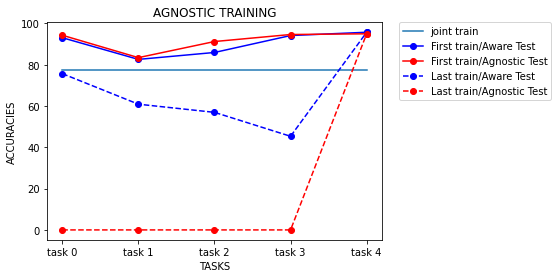
\includegraphics[width=\linewidth]{Agnostic_Agnostic-Aware.png}
\label{figure : Angostic_training}
\end{figure}
\newpage
Prima di analizzare il grafico  andiamo a considerare il paradigma l'\textit{Agnostic-Training} che consiste nel \textit{Training}
senza sapere di quale \textit{Task} ci stiamo occupando.
Ciò comporta che ad ogni \textit{Task} l'output della rete consisterà in tutti i moduli dei \textit{Tasks} fino a quello corrente concatenati nel metodo \textit{Forward}, questo perchè non possiamo selezionare l'\textit{output} relativo al \textit{Task} in esecuzione.
\newline
Dal grafico ~\ref{figure : Angostic_training}, che si trova a pagina precendete, possiamo notare vari aspetti interessanti sui risultati ottenuti. Prima di tutto, notiamo che i valori delle \textit{accuarcies} sui vari \textit{Tasks} calcolate dopo i rispettivi \textit{Training} ottengono valori molto elevati che superano persino il valore del \textit{Joint Train}. Questo è dovuto al numero minore di dati utilizzati rispetto al \textit{Dataset} completo e dal fatto che il \textit{Test} è effetuato subito  dopo il \textit{Training} del relativo \textit{Task}. Inoltre, da notare, come i due approcci di \textit{Testing} ottengano \textit{accuracies} quasi identiche, questo perchè la rete viene \textit{testata} subito dopo il \textit{train} relativo di conseguenza i pesi associati alla clasificazione sono molto precisi per entrambe le configurazioni, ottenendo risulati, per ciascun \textit{Task}, migliori anche del \textit{Joint Train} .
L'\textit{accuracy} calcolata sull'ultimo \textit{task}, naturalmente, avrà valore uguale per tutte e quattro le configurazioni, come si può nel grafico ~\ref{figure : Angostic_training} nel punto relativo a quest'ultimo.
\newline
Per quanto riguarda le \textit{accuracies} calcolate successivamente all'ultimo\textit{Training}, vediamo che otteniamo un calo drastico di precisione su ciasciun \textit{Task} escluso l'ultimo come abbiamo precedentemente notato. Questo è il fenomeno del \textbf{Catastrophic Forgetting}, introdotto nel \autoref{ch:chapter1}, che porta il \textit{modello} a dimenticare tutti i \textit{weight} relativi ai \textit{Tasks} precedenti.
In Particolare nella configurazione Aware otteniamo dei valori migliori dati dall'output più preciso e specifico per il relativo \textit{Task}, ottenuto selezionando la \textit{Classification Head} realtiva a quest'ultimo. Per quanto riguarda la configurazione di \textit{Agnostic Testing}, otteniamo un valore molto alto per l'ultimo \textit{Task} mentre per i 4 precedenti l'\textit{accuracy} va a 0. Queto fenomeno prende il nome di 
\textit{\textbf{Task Recency Bias}}. Si tratta di un fenomeno che consiste nel fatto che la \textit{rete} tenda a ricordare e a prevedere meglio dati su cui è stato fatto per ultimo il \textit{Training} portando a dimenticare totalmente i \textit{Tasks} precedenti, come viene descritto in \textbf{FARE CITAZIONE AL PAPER}. Questo risultato è rincondotto all'utilizzo di \textit{CrossEntropyLoss}  che aumenta il valore della probabibiltà relativa alla classe corretta e abbassa quella relativa alla classe non corretta all'interno della distribuzione di probabilità, siccome grazie al \textit{SoftMax} la somma dei valori deve essere uguale a uno. Ad ogni esempio del batch del \textit{Task} corrente butta giù la probabilità delle classi appartenenti a quelli precedenti andando incontro al \textbf{Catastrophic Forgetting}.
\newline
Per questo motivo è interessante valutare le medie delle \textit{accuracies} per analizzare l'occorrere del \textbf{Catastrophic Forgetting} nelle varie configurazioni.
Qui di seguito i valori delle accuracy riporatet in due tabelle, una per tipologia di \textit{Testing}.
\begin{table}[!htb]
\begin{minipage}{.5\linewidth}
    \centering

    \label{tab:Agnostic-Agnostic }

    \medskip

\begin{tabular}{l*{6}{c}r}
Tasks   & First Train & Last Train\\
\hline
   Task 0      &     94.30      &      0.0\\
   Task 1      &     83.45      &      0.0\\
   Task 2      &     91.25      &      0.0\\
   Task 3      &     94.65      &      0.0\\
   Task 4      &     95.00      &      95.00\\
\end{tabular}
\caption{Agnostic-Agnostic}
\label{tab:Agnostic-Agnostic}
\end{minipage}\hfill
\begin{minipage}{.5\linewidth}
    \centering

    \label{tab:Agnostic-Aware}

    \medskip

\begin{tabular}{l*{6}{c}r}
Tasks   & First Train  & Last Train\\
\hline
   Task 0      &     93.10      &      75.70\\
   Task 1      &     82.60      &      60.90\\
   Task 2      &     85.95      &      56.95\\
   Task 3      &     94.15      &      45.35\\
   Task 4      &     95.75      &      95.75\\
\end{tabular}
\caption{Agnostic-Aware}
\label{tab:Agnostic-Aware}
\end{minipage}
\end{table}
\newline
Nelle tabelle~\ref{tab:Agnostic-Agnostic} e~\ref{tab:Agnostic-Aware} notiamo, come avevamo già fatto nel grafico in figura ~\ref{figure : Angostic_training} a pagina ~\pageref{figure : Angostic_training}, che l'\textit{accuracy} della configurazione \textit{Agnostic-Agnostic} è peggiore rispetto a quella di \textit{Agnostic-Aware} ma per valutare la differenza di valori, ma soprattutto il \textit{Forgetting}, calcoliamo la media i quest'ultimi.
\newline
Facendo le medie otteniamo i seguenti valori:
\begin{itemize}
    \item Tabella~\ref{tab:Agnostic-Agnostic}: Abbiamo una \textit{accuracy} iniziale di 91.73\% e finale del 19.0\%, quindi otteniamo un decremento del 72.71\%.
    \item Tabella~\ref{tab:Agnostic-Aware}: Abbiamo una \textit{accuracy} iniziale di 90.30\% e finale del 66.92\%, quindi otteniamo un decremento del 23.38\%.
\end{itemize}
Notiamo che la media dell'\textit{accuracy} del \textit{Task Agnostic} e \textit{Task Aware Testing} sono entrambe inferiori dell'\textit{Upperbound} rappresentato dal \textit{Joint-Train}, confermando ciò che si poteva notare già a livello grafico nell'immagine~\ref{figure : Angostic_training}.
Il decremento della \textit{accuracy} ci serve a valutare l'entità del \textit{Catastrophic Forgetting} a cui siamo andati incontro.
\newline
Questo valore inoltre ci conferma il \textit{forgetting} molto elevato che abbiamo ottenuto sui \textit{Tasks} precedenti all'ultimo  utilizzando la configurazione \textit{Agnostic-Agnostic}. Vedremo successivamente una soluzione naive al problema del \textit{Task Recency Bias}(che colpisce in minor modo la configurazione \textit{Agnostic-Aware}), basato sull'approccio \textit{Replay Based Methods}.
\newline
In generale il decremento di \textit{accuracy} per entrambe le configurazioni utilizzate in questo paragrafo, è elevato anche se con entità diverse. Inoltre la distanza di \textit{accuracy} in media dal valore ottenuto con il \textit{Joint-Train} assume un valore del 10,68\%, per la configurazione \textit{Agnostic-Aware}, 58,60\% per \textit{Agnostic-Agnostic}. Questo ci fa comprendere l'entità del \textit{drop} di \textit{accuracy} a cui si può andare incontro adottando una divisione in \textit{Tasks} dovuto al \textit{catastrophic forgetting}.
\subsection{Aware-training}
In queta sezione ci concentriamo su altre due configurazioni\textit{Task-Aware} per il \textit{Training} introdotte già a \textit{pag.} 14.
A differenza della configurazione \textit{Task-Aware} possiamo selezionare la \textit{Classification Head} relativa al \textit{Task} corrrente, di conseguenza il \textit{Training} per ognuno di essi sarà eseguito con un \textit{output} di soli due valori modificando quindi l'aggiornamento dei parametri della \textit{Rete}.\newline
Riportiamo qui di seguito il grafico che rappresenta le accuracy:
\begin{figure}[ht]
\centering
\caption{Agnostic Training}
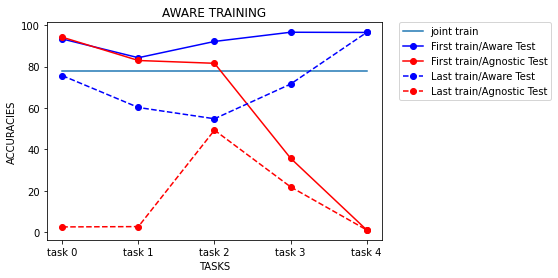
\includegraphics[width=\linewidth]{Aware_Agnostic-Aware.png}
\label{figure : Aware_Training}
\end{figure}
\newline
Dalla figura ~\ref{figure : Aware_Training} possiamo notare che l'andamento generale delle accuracy segue, in linea generale, quello della figura ~\ref{figure : Angostic_training} a pagina 15.
Di conseguenza abbiamo che l'\textit{accuracy} su un \textit{Task} calcolata subito dopo il corrispondente addestramento ha un valore molto buono, che in media è addirittura superiore al \textit{Joint Train}, sia per \textit{Aware} che \textit{Agnostic Test}. Inoltre abbiamo che l'accuracy sull'ultimo \textit{Task} ha lo stesso valore per tutti i casi riportati, tranne uno \textit{Aware-Agnostic}. Si può notare che l'\textit{accuracy} calcolata sull'ultimo \textit{Task} a seconda della tipologia assume dei valori diversi.
In particolare la configurazione \textit{Agnostic Test} notiamo che l'accuracy subito dopo il \textit{Training} assume un valore sempre minore fino all'ultimo \textit{Task} in cui è quasi nulla. Questo risultato è ottenuto perchè durante la fase \textit{Train} utilizziamo la \textit{classification head} specifica del \textit{Task} mentre nella fase di \textit{Testing} utilizziamo un \textit{output} unico per tutti \textit{Tasks} fino a quello corrente.
Adesso mostriamo di seguito la tabella con le accuracy ottenute per poter capire il \textit{forgetting} ottenuto e comparare i risultati con l' \textit{Agnostic Train}:
\begin{table}[!htb]
\begin{minipage}{.5\linewidth}
    \centering

    \label{tab:Aware-Agnostic }

    \medskip

\begin{tabular}{l*{6}{c}r}
Tasks   & First Train & Last Train\\
\hline
   Task 0      &     94.15      &       2.50\\
   Task 1      &     82.90      &       2.65\\
   Task 2      &     81.55      &      49.25\\
   Task 3      &     35.70      &      21.85\\
   Task 4      &      1.05      &       1.05\\
\end{tabular}
\caption{Aware-Agnostic}
\label{tab:Aware-Agnostic}
\end{minipage}\hfill
\begin{minipage}{.5\linewidth}
    \centering

    \label{tab:Aware-Aware}

    \medskip

\begin{tabular}{l*{6}{c}r}
Tasks   & First Train  & Last Train\\
\hline
   Task 0      &     93.30      &      75.60\\
   Task 1      &     84.25      &      60.20\\
   Task 2      &     92.10      &      54.75\\
   Task 3      &     96.55      &      71.50\\
   Task 4      &     96.45      &      96.45\\
\end{tabular}
\caption{Aware-Aware}
\label{tab:Aware-Aware}
\end{minipage}
\end{table}
\newline
Nelle tabelle ~\ref{tab:Aware-Agnostic} e ~\ref{tab:Aware-Aware} notiamo subito che la accuracy rilevata nel caso di \textit{Aware Testing} è migliore, ma consideriamo adesso le medie delle \textit{accuracies} e il \textit{Forgetting} ottenuto.
\begin{itemize}
    \item Tabella~\ref{tab:Aware-Agnostic}: Abbiamo una \textit{accuracy} iniziale di 59.07\% e finale del 15.45\%, quindi otteniamo un decremento del 43.61\%.
    \item Tabella~\ref{tab:Aware-Aware}: Abbiamo una \textit{accuracy} iniziale di 92.53\% e finale del 71.7\%, quindi otteniamo un decremento del 20.83\%.
\end{itemize}
La prima cosa che notiamo è che l'accuracy iniziale della configurazione \textit{Agnostic-Agnostic} ha ottenuto un valore in media molto minore rispetto alle altre causato dall'\textit{Agnostic Testing}.
L'accuracy ottenuta nel caso \textit{Aware-Aware} è il miglior risultato e si avvicina a quella del \textit{Joint-Train} con uno scarto del 5,9\%. Mentre nel caso della Tabella ~\ref{tab:Aware-Agnostic} l'\textit{Accuracy} ottenuta rappresenta il \textit{Lower-Bound} dei risultati con uno scarto dal \textit{Joint-Train} del 62,15\%. 
\section{Soluzione Naïve}
In questa sezione andiamo ad proporre una soluzione con un \textit{naïve} al probelma del \textit{Catastrophic Forgetting}. Esistono tre famiglie di soluzioni al problema del \textit{Continual Learning}:
\begin{itemize}
    \item \textit{Replay methods}
    \item \textit{Regularization-based methods}
    \item\textit{Parameter isolation methods}
\end{itemize}
In questa sezione ci soffermeremo su una soluzione \textit{Naïve} dellla famiglia dei \textit{\textbf{Replay methods}}. Questo approccio consiste nel memorizzare i campioni o generare \textit{pseudo-campioni} con un modello generativo appartenenti ai \textit{Tasks} precedenti. Questi esempi  vengono riutilizzati durante l'apprendimento di un nuovo \textit{Task} per alleviare il \textit{Forgetting}.\newline
Il problema principale dei \textit{Replay methods} risiede nella memoria, salvando esempi dai \textit{Task} precendeti la memori necessaria a ciascun \textit{Task} sarà sempre maggiore. Ciò può esser ovviato utiizzando un limite di esempi possibili dai precedenti \textit{Tasks} ottenendo però una perdita di generalizzazione del rispettivo \textit{Task}.
PARLARE IN BREVE DEI METODI GEM E ICARL E SUCCESSIVAMENTE DELLA SCELTA NAIVE
\chapter{Conclusioni}\label{ch:conclusioni}
\section{Risultati}
Il lavoro che è stato descritto in questo elaborato di tesi può essere ritenuto soddisfacente. Il nostro intento era quello di rappresentare al meglio il \textbf{Continual Learning} e il suo problema del \textbf{Catastrophic Forgetting}, perciò nella nostra \textit{pipeline} non è stato inserito nessun metodo che potesse alleviare o bloccare tale problema. Abbiamo potuto osservare come il \textit{training} effettuato in fasi diverse per ciascun \textit{task} abbia portato al \textit{forgetting}, valutandolo sia nel caso \textit{Task-Aware} che \textit{Task-Agnostic}.\newline
È stato riscontrato un \textit{forgetting} minore nelle configurazioni in cui è stato applicato il \textit{Task-Aware Test}, peggiore con \textit{Task-Agnostic Test}. Per questo motivo è stato scelto come caso interessante, su cui applicare una soluzione basata \textit{Replay-Based Methods}, \textit{Task-Agnostic Training/Task-Agnostic Test}.
Con tale soluzione è stato possibile ottenere dei risultati migliori rispetto ai precedenti. Infatti, questa configurazione soffriva del \textit{Task Rececncy Bias} che portava a dimenticare completamente i parametri dei \textit{tasks} precedenti all'ultimo visionato. Usando un numero di esempi limitato per fare il \textit{replay} siamo riusciti ad avvicinarci al \textit{Joint-Train}, mantenendo comunque un \textit{forgetting} elevato.
La rete neurale sviluppata non è ovviamente \textbf{immune} da \textbf{errori}, potrebbero essere apportate delle migliorie in modo tale da adattarsi meglio al problema in esame, ottenendo  risultati migliori.
\section{Sviluppi Futuri}
Negli esperimenti eseguiti in questo elaborato, abbiamo considerato un ambiente di apprendimento basato sul concetto \textit{Task Incremental}. In questo \textit{setting} i \textit{tasks} vengono ricevuti sequenzialmente e il \textit{Training}  viene eseguito sui dati di addestramento associati. È, quindi, richiesta la conoscenza dei limiti dei \textit{tasks} (ovvero quando i \textit{tasks} cambiano), consentendo più passaggi su grandi \textit{batch} di dati di \textit{training}. Può essere, quindi, un rilassamento del sistema di \textit{Continual Learning} desiderato che è più probabile incontrare nella pratica. Una evoluzione potrebbe essere quella di rendere il modello capace di processare dati di \textit{tasks} diversi senza considerarne i limiti, al fine di riconoscere se l'\textit{input} appartiene a un \textit{task} già osservato. Questa modifica potrebbe conferire grande flessibilità al metodo del \textit{Continual Learning} rendendolo applicabile a qualsiasi scenario in cui i dati arrivano con uno \textit{stream} infinito.
\newline
Un altro sviluppo possibile, potrebbe essere quello di utilizzare un dataset diverso. Sarebbe appunto interessante osservare i risultati all'aumentare del numero di classi presenti nel dataset, o altrimenti, all'aumentare del numero di esempi presenti nel \textit{trainset} e \textit{testset}. Un dataset che viene spontaneamente in mente dopo la lettura di questo elaborato è \textit{CIFAR-100}. Quest'ultimo non è altro che una estensione di \textit{CIFAR-10}(utilizzato in questo elaborato), composto da 100 \textit{classi} differenti. Tale modifica ci consentirebbe di visualizzare più \textit{tasks} e con un numero di classi associato maggiore.\newline
Infine, nella soluzione che abbiamo esposto per alleviare il \textit{forgetting} non è stata attuata nessuna tecnica per sceglie gli esempi su cui fare il \textit{replay}, quindi una direzione di sviluppo potrebbe essere questa. Come viene descritto in \cite{Continual_Learning}, esistono dei metodi specifici del \textbf{Reaplay Based Methods}:
\textit{iCaRL} e \textit{GEM}. In particolare, questi due metodi attuano delle politiche per la scelta degli esempi utilizzati nel \textit{replay}.
\textit{iCaRL} si basa sulla stima della \textit{Loss}, mentre \textit{GEM} si concentra sul \textit{gradiente}.

\addcontentsline{toc}{chapter}{Bibliografia}
\bibliographystyle{unsrt}
\bibliography{files/biblio}
%\bibliography{sp,xml}
%\bibliographystyle{ieeetr}
%\bibliography{sp,xml}

\end{document} 

